%!TeX root=../pridetop.tex
\chapter[Chapter \thechapter]{}
	
	
\begin{figure}[t!]
\centering
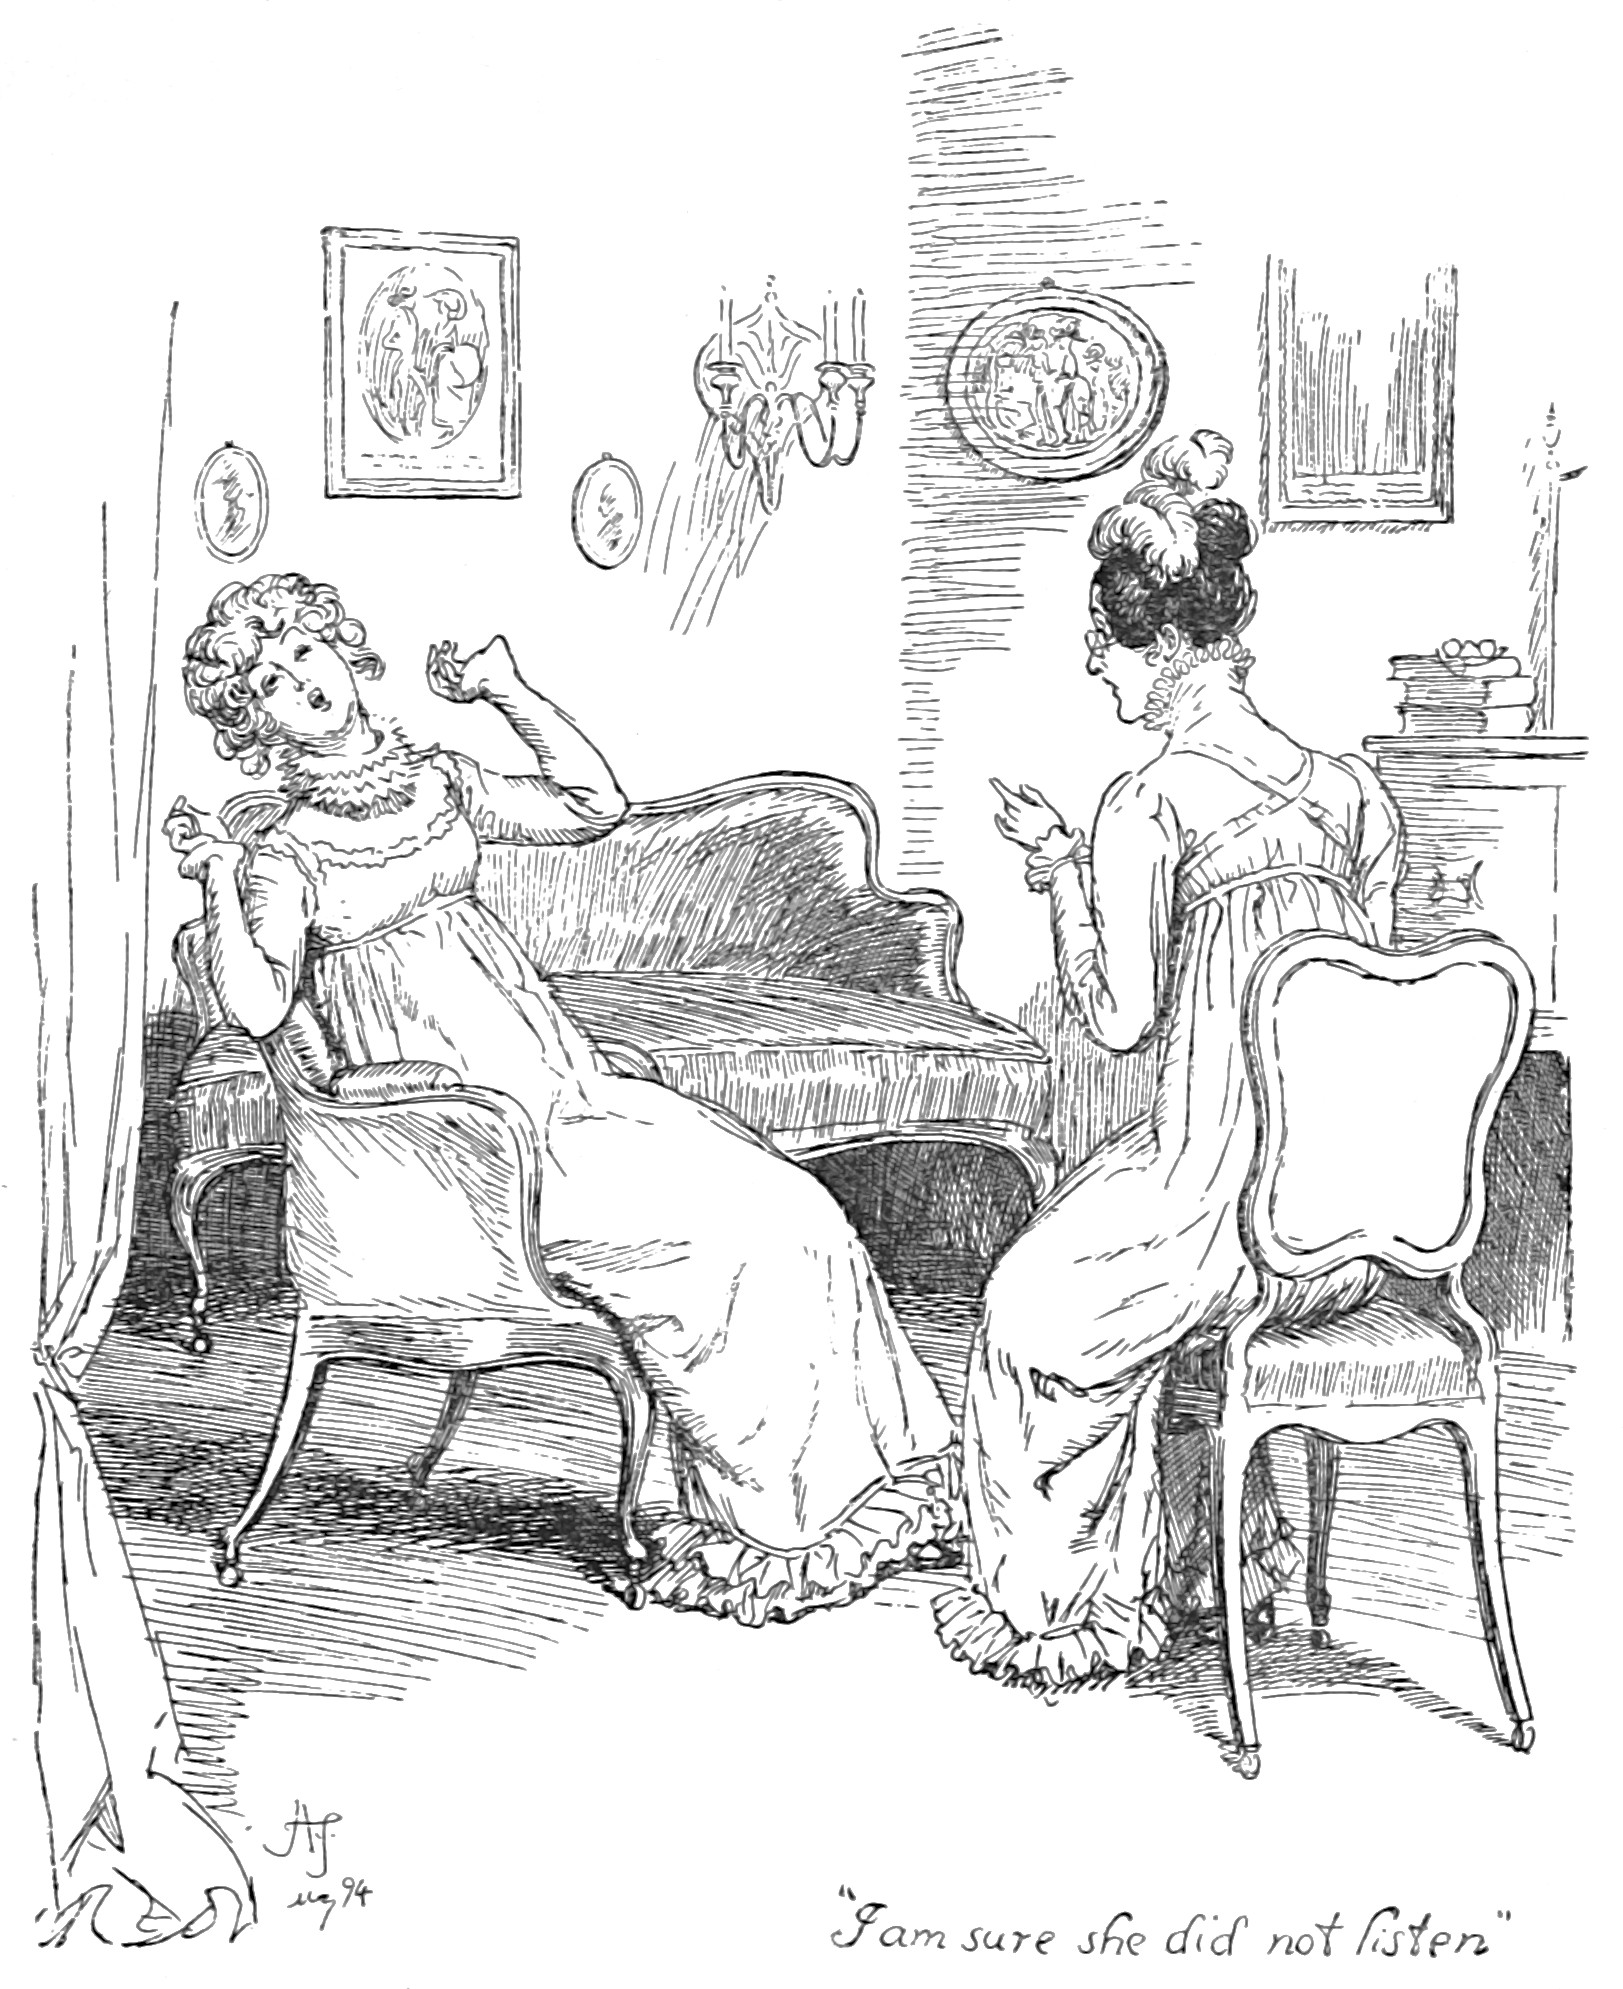
\includegraphics[width=.85\linewidth]{52top}
\captionlistentry{<I am sure she did not listen>}
\end{figure}


\lettrine[lines=6,image=true]{initials/chap52e}{lizabeth}  had the satisfaction of receiving an answer to her letter as soon as she possibly could. She was no sooner in possession of it, than hurrying into the little copse, where she was least likely to be interrupted, she sat down on one of the benches, and prepared to be happy; for the length of the letter convinced her that it did not contain a denial.

\begin{mail}{Gracechurch Street\\ Sept. 6.}{My dear Niece,}

I have just received your letter, and shall devote this whole morning to answering it, as I foresee that a \textit{little} writing will not comprise what I have to tell you. I must confess myself surprised by your application; I did not expect it from \textit{you}. Don't think me angry, however, for I only mean to let you know, that I had not imagined such inquiries to be necessary on \textit{your} side. If you do not choose to understand me, forgive my impertinence. Your uncle is as much surprised as I am; and nothing but the belief of your being a party concerned would have allowed him to act as he has done. But if you are really innocent and ignorant, I must be more explicit. On the very day of my coming home from Longbourn, your uncle had a most unexpected visitor. Mr Darcy called, and was shut up with him several hours. It was all over before I arrived; so my curiosity was not so dreadfully racked as \textit{yours} seems to have been. He came to tell Mr Gardiner that he had found out where your sister and Mr Wickham were, and that he had seen and talked with them both—Wickham repeatedly, Lydia once. From what I can collect, he left Derbyshire only one day after ourselves, and came to town with the resolution of hunting for them. The motive professed was his conviction of its being owing to himself that Wickham's worthlessness had not been so well known as to make it impossible for any young woman of character to love or confide in him. He generously imputed the whole to his mistaken pride, and confessed that he had before thought it beneath him to lay his private actions open to the world. His character was to speak for itself. He called it, therefore, his duty to step forward, and endeavour to remedy an evil which had been brought on by himself. If he \textit{had another} motive, I am sure it would never disgrace him. He had been some days in town before he was able to discover them; but he had something to direct his search, which was more than \textit{we} had; and the consciousness of this was another reason for his resolving to follow us. There is a lady, it seems, a Mrs Younge, who was some time ago governess to Miss Darcy, and was dismissed from her charge on some cause of disapprobation, though he did not say what. She then took a large house in Edward Street, and has since maintained herself by letting lodgings. This Mrs Younge was, he knew, intimately acquainted with Wickham; and he went to her for intelligence of him, as soon as he got to town. But it was two or three days before he could get from her what he wanted. She would not betray her trust, I suppose, without bribery and corruption, for she really did know where her friend was to be found. Wickham, indeed, had gone to her on their first arrival in London; and had she been able to receive them into her house, they would have taken up their abode with her. At length, however, our kind friend procured the wished-for direction. They were in — Street. He saw Wickham, and afterwards insisted on seeing Lydia. His first object with her, he acknowledged, had been to persuade her to quit her present disgraceful situation, and return to her friends as soon as they could be prevailed on to receive her, offering his assistance as far as it would go. But he found Lydia absolutely resolved on remaining where she was. She cared for none of her friends; she wanted no help of his; she would not hear of leaving Wickham. She was sure they should be married some time or other, and it did not much signify when. Since such were her feelings, it only remained, he thought, to secure and expedite a marriage, which, in his very first conversation with Wickham, he easily learnt had never been \textit{his} design. He confessed himself obliged to leave the regiment on account of some debts of honour which were very pressing; and scrupled not to lay all the ill consequences of Lydia's flight on her own folly alone. He meant to resign his commission immediately; and as to his future situation, he could conjecture very little about it. He must go somewhere, but he did not know where, and he knew he should have nothing to live on. Mr Darcy asked why he did not marry your sister at once. Though Mr Bennet was not imagined to be very rich, he would have been able to do something for him, and his situation must have been benefited by marriage. But he found, in reply to this question, that Wickham still cherished the hope of more effectually making his fortune by marriage, in some other country. Under such circumstances, however, he was not likely to be proof against the temptation of immediate relief. They met several times, for there was much to be discussed. Wickham, of course, wanted more than he could get; but at length was reduced to be reasonable. Everything being settled between \textit{them}, Mr Darcy's next step was to make your uncle acquainted with it, and he first called in Gracechurch Street the evening before I came home. But Mr Gardiner could not be seen; and Mr Darcy found, on further inquiry, that your father was still with him, but would quit town the next morning. He did not judge your father to be a person whom he could so properly consult as your uncle, and therefore readily postponed seeing him till after the departure of the former. He did not leave his name, and till the next day it was only known that a gentleman had called on business. On Saturday he came again. Your father was gone, your uncle at home, and, as I said before, they had a great deal of talk together. They met again on Sunday, and then \textit{I} saw him too. It was not all settled before Monday: as soon as it was, the express was sent off to Longbourn. But our visitor was very obstinate. I fancy, Lizzy, that obstinacy is the real defect of his character, after all. He has been accused of many faults at different times; but \textit{this} is the true one. Nothing was to be done that he did not do himself; though I am sure (and I do not speak it to be thanked, therefore say nothing about it) your uncle would most readily have settled the whole. They battled it together for a long time, which was more than either the gentleman or lady concerned in it deserved. But at last your uncle was forced to yield, and instead of being allowed to be of use to his niece, was forced to put up with only having the probable credit of it, which went sorely against the grain; and I really believe your letter this morning gave him great pleasure, because it required an explanation that would rob him of his borrowed feathers, and give the praise where it was due. But, Lizzy, this must go no further than yourself, or Jane at most. You know pretty well, I suppose, what has been done for the young people. His debts are to be paid, amounting, I believe, to considerably more than a thousand pounds, another thousand in addition to her own settled upon \textit{her}, and his commission purchased. The reason why all this was to be done by him alone, was such as I have given above. It was owing to him, to his reserve and want of proper consideration, that Wickham's character had been so misunderstood, and consequently that he had been received and noticed as he was. Perhaps there was some truth in \textit{this}; though I doubt whether \textit{his} reserve, or \textit{anybody's} reserve can be answerable for the event. But in spite of all this fine talking, my dear Lizzy, you may rest perfectly assured that your uncle would never have yielded, if we had not given him credit for \textit{another interest} in the affair. When all this was resolved on, he returned again to his friends, who were still staying at Pemberley; but it was agreed that he should be in London once more when the wedding took place, and all money matters were then to receive the last finish. I believe I have now told you everything. It is a relation which you tell me is to give you great surprise; I hope at least it will not afford you any displeasure. Lydia came to us, and Wickham had constant admission to the house. \textit{He} was exactly what he had been when I knew him in Hertfordshire; but I would not tell you how little I was satisfied with \textit{her} behaviour while she stayed with us, if I had not perceived, by Jane's letter last Wednesday, that her conduct on coming home was exactly of a piece with it, and therefore what I now tell you can give you no fresh pain. I talked to her repeatedly in the most serious manner, representing to her the wickedness of what she had done, and all the unhappiness she had brought on her family. If she heard me, it was by good luck, for I am sure she did not listen. I was sometimes quite provoked; but then I recollected my dear Elizabeth and Jane, and for their sakes had patience with her. Mr Darcy was punctual in his return, and, as Lydia imformed you, attended the wedding. He dined with us the next day, and was to leave town again on Wednesday or Thursday. Will you be very angry with me, my dear Lizzy, if I take this opportunity of saying (what I was never bold enough to say before) how much I like him? His behaviour to us has, in every respect, been as pleasing as when we were in Derbyshire. His understanding and opinions all please me; he wants nothing but a little more liveliness, and \textit{that}, if he marry \textit{prudently}, his wife may teach him. I thought him very sly; he hardly ever mentioned your name. But slyness seems the fashion. Pray forgive me, if I have been very presuming, or at least do not punish me so far as to exclude me from P. I shall never be quite happy till I have been all round the park. A low phaeton with a nice little pair of ponies would be the very thing. But I must write no more. The children have been wanting me this half hour.

\closeletter[Yours, very sincerely,]{M. Gardiner.}

\end{mail}

The contents of this letter threw Elizabeth into a flutter of spirits, in which it was difficult to determine whether pleasure or pain bore the greatest share. The vague and unsettled suspicions which uncertainty had produced, of what Mr Darcy might have been doing to forward her sister's match—which she had feared to encourage, as an exertion of goodness too great to be probable, and at the same time dreaded to be just, from the pain of obligation—were proved beyond their greatest extent to be true! He had followed them purposely to town, he had taken on himself all the trouble and mortification attendant on such a research; in which supplication had been necessary to a woman whom he must abominate and despise, and where he was reduced to meet, frequently meet, reason with, persuade, and finally bribe the man whom he always most wished to avoid, and whose very name it was punishment to him to pronounce. He had done all this for a girl whom he could neither regard nor esteem. Her heart did whisper that he had done it for her. But it was a hope shortly checked by other considerations; and she soon felt that even her vanity was insufficient, when required to depend on his affection for her, for a woman who had already refused him, as able to overcome a sentiment so natural as abhorrence against relationship with Wickham. Brother-in-law of Wickham! Every kind of pride must revolt from the connection. He had, to be sure, done much. She was ashamed to think how much. But he had given a reason for his interference, which asked no extraordinary stretch of belief. It was reasonable that he should feel he had been wrong; he had liberality, and he had the means of exercising it; and though she would not place herself as his principal inducement, she could perhaps believe, that remaining partiality for her might assist his endeavours in a cause where her peace of mind must be materially concerned. It was painful, exceedingly painful, to know that they were under obligations to a person who could never receive a return. They owed the restoration of Lydia, her character, everything to him. Oh, how heartily did she grieve over every ungracious sensation she had ever encouraged, every saucy speech she had ever directed towards him! For herself she was humbled; but she was proud of him,—proud that in a cause of compassion and honour he had been able to get the better of himself. She read over her aunt's commendation of him again and again. It was hardly enough; but it pleased her. She was even sensible of some pleasure, though mixed with regret, on finding how steadfastly both she and her uncle had been persuaded that affection and confidence subsisted between Mr Darcy and herself.

She was roused from her seat and her reflections, by someone's approach; and, before she could strike into another path, she was overtaken by Wickham.

<I am afraid I interrupt your solitary ramble, my dear sister?> said he, as he joined her.

<You certainly do,> she replied with a smile; <but it does not follow that the interruption must be unwelcome.>

<I should be sorry, indeed, if it were. \textit{We} were always good friends, and now we are better.>

<True. Are the others coming out?>

<I do not know. Mrs Bennet and Lydia are going in the carriage to Meryton. And so, my dear sister, I find, from our uncle and aunt, that you have actually seen Pemberley.>

She replied in the affirmative.

<I almost envy you the pleasure, and yet I believe it would be too much for me, or else I could take it in my way to Newcastle. And you saw the old housekeeper, I suppose? Poor Reynolds, she was always very fond of me. But of course she did not mention my name to you.>

<Yes, she did.>

<And what did she say?>

<That you were gone into the army, and she was afraid had—not turned out well. At such a distance as \textit{that}, you know, things are strangely misrepresented.>

<Certainly,> he replied, biting his lips. Elizabeth hoped she had silenced him; but he soon afterwards said,—

<I was surprised to see Darcy in town last month. We passed each other several times. I wonder what he can be doing there.>

<Perhaps preparing for his marriage with Miss de Bourgh,> said Elizabeth. <It must be something particular to take him there at this time of year.>

<Undoubtedly. Did you see him while you were at Lambton? I thought I understood from the Gardiners that you had.>

<Yes; he introduced us to his sister.>

<And do you like her?>

<Very much.>

<I have heard, indeed, that she is uncommonly improved within this year or two. When I last saw her, she was not very promising. I am very glad you liked her. I hope she will turn out well.>

<I dare say she will; she has got over the most trying age.>

<Did you go by the village of Kympton?>

<I do not recollect that we did.>

<I mention it because it is the living which I ought to have had. A most delightful place! Excellent parsonage-house! It would have suited me in every respect.>

<How should you have liked making sermons?>

<Exceedingly well. I should have considered it as part of my duty, and the exertion would soon have been nothing. One ought not to repine; but, to be sure, it would have been such a thing for me! The quiet, the retirement of such a life, would have answered all my ideas of happiness! But it was not to be. Did you ever hear Darcy mention the circumstance when you were in Kent?>

<I \textit{have} heard from authority, which I thought \textit{as good}, that it was left you conditionally only, and at the will of the present patron.>

<You have! Yes, there was something in \textit{that}; I told you so from the first, you may remember.>

<I \textit{did} hear, too, that there was a time when sermon-making was not so palatable to you as it seems to be at present; that you actually declared your resolution of never taking orders, and that the business had been compromised accordingly.>

<You did! and it was not wholly without foundation. You may remember what I told you on that point, when first we talked of it.>

They were now almost at the door of the house, for she had walked fast to get rid of him; and unwilling, for her sister's sake, to provoke him, she only said in reply, with a good-humoured smile,—

<Come, Mr Wickham, we are brother and sister, you know. Do not let us quarrel about the past. In future, I hope we shall be always of one mind.>

She held out her hand: he kissed it with affectionate gallantry, though he hardly knew how to look, and they entered the house.